% Exam Template for UMTYMP and Math Department courses
%
% Using Philip Hirschhorn's exam.cls: http://www-math.mit.edu/~psh/#ExamCls
%
% run pdflatex on a finished exam at least three times to do the grading table on front page.
%
%%%%%%%%%%%%%%%%%%%%%%%%%%%%%%%%%%%%%%%%%%%%%%%%%%%%%%%%%%%%%%%%%%%%%%%%%%%%%%%%%%%%%%%%%%%%%%

% These lines can probably stay unchanged, although you can remove the last
% two packages if you're not making pictures with tikz.
\documentclass[11pt]{exam}
\RequirePackage{amssymb, amsfonts, amsmath, latexsym, verbatim, xspace, setspace}
\RequirePackage{tikz, pgflibraryplotmarks}
\RequirePackage{hyperref}
\usepackage{graphicx}
\usepackage{caption}
\usepackage{subcaption}


\def\QED{\ensuremath{{\square}}}
\def\markatright#1{\leavevmode\unskip\nobreak\quad\hspace*{\fill}{#1}}
\newenvironment{proof}
  {\begin{trivlist}\item[\hskip\labelsep{\bf Proof.}]}
  {\markatright{\QED}\end{trivlist}}


% By default LaTeX uses large margins.  This doesn't work well on exams; problems
% end up in the "middle" of the page, reducing the amount of space for students
% to work on them.
\usepackage[margin=1in]{geometry}


% Here's where you edit the Class, Exam, Date, etc.
\newcommand{\class}{Christmas 101}
\newcommand{\term}{Fall 2015}
\newcommand{\examnum}{Exam 1}
\newcommand{\examdate}{December 25, 2015}
\newcommand{\timelimit}{180 Minutes}

% For an exam, single spacing is most appropriate
\singlespacing
% \onehalfspacing
% \doublespacing

% For an exam, we generally want to turn off paragraph indentation
\parindent 0ex

\begin{document}

% These commands set up the running header on the top of the exam pages
\pagestyle{head}
\firstpageheader{}{}{}
\runningheader{\class}{\examnum\ - Page \thepage\ of \numpages}{\examdate}
\runningheadrule

\begin{flushright}
\begin{tabular}{p{2.8in} r l}
\textbf{\class} & \textbf{Name (Print):} & \makebox[2in]{\hrulefill}\\
\textbf{\term} &&\\
\textbf{\examnum} &&\\
\textbf{\examdate} &&\\
\textbf{Time Limit: \timelimit} & % Teaching Assistant & \makebox[2in]{\hrulefill}
\end{tabular}\\
\end{flushright}
\rule[1ex]{\textwidth}{.1pt}

Welcome to the third year of the ongoing tradition of making Beingessner(s)
Edward and Holly work for the Christmas presents they receive from
Beingessner(s) Julia, Sonia and Alexis, and Collymore, Mike.
\vspace{1cm}

This year, the challenge is a multi-subject exam. Each point earned on the exam
is equal to 50 Canadian cents. A total of 120 points can be earned on the exam
proper, and there are also bonus questions.
\vspace{1cm}

Only one test may be taken per examinee. Examinees may not communicate with each
other, or with anyone other than the official exam proctors (Beingessner(s)
Julia, Sonia and Alexis, and Collymore, Mike). All electronic devices will be
confiscated, including laptops, tablets, desktop computers, fancy watches, time
machines, cellphones, etc.

Cheating on the exam will disqualify the examinee from receiving any money.

This exam is open book. The following resources may be used:

\begin{enumerate}
\item Beingessner, Sean P. ``A study of the gain mechanism of gas filled proportional wire counters.'' PhD diss., Carleton University, 1984.

\item Beingessner, Sonia. ``Self portrait R\&R.'' Illustration. 2015. From the artist’s personal Facebook account. \
% url{https://www.facebook.com/photo.php?fbid=10153710069418659&set=rpd.510703658&type=3&theater}
(accessed December 23, 2015).

\item Beingessner, Sonia. ``The band in uncharted territory.'' Illustration. 2015. From the artist’s personal website.
% \url{http://vaniabogue.blogspot.ca/2015/09/self-portrait-r-self-portrait-in-style.html}
% (accessed December 23, 2015).

\item Collymore, Mike. ``Starcrossed.'' Comic. 2015. From the artist’s personal website.
% \url{http://mikecollymore.blogspot.ca/2015/11/starcrossed-inktober-2015.html}
(accessed December 23, 2015).

\item The Rust Team. \emph{The Rustonomicon}: The Dark Arts of Advanced and Unsafe Rust Programming. Draft documentation, 2015.
% \url{https://killercup.github.io/trpl-ebook/nomicon-2015-09-12.a4.pdf}
(accessed: December 23, 2015).

\item Beingessner, Julia. ``There is no Manchukuo.'' Essay, McGill University, 2009.

\item Beingessner, Julia. ``Web Services' Guide to Web Accessibility and Technical Requirements.''
Ottawa, Treasury Board of Canada Secretariat, 2012. © Her Majesty the Queen in Right of
Canada.
\end{enumerate}

Calculators are forbidden in this exam, with the exception of:

\begin{itemize}
\item Sean Beingessner's Polish reverse polarization calculator from 1975.
\end{itemize}




\newpage % End of cover page

%%%%%%%%%%%%%%%%%%%%%%%%%%%%%%%%%%%%%%%%%%%%%%%%%%%%%%%%%%%%%%%%%%%%%%%%%%%%%%%%%%%%%
%
% See http://www-math.mit.edu/~psh/#ExamCls for full documentation, but the questions
% below give an idea of how to write questions [with parts] and have the points
% tracked automatically on the cover page.
%
%
%%%%%%%%%%%%%%%%%%%%%%%%%%%%%%%%%%%%%%%%%%%%%%%%%%%%%%%%%%%%%%%%%%%%%%%%%%%%%%%%%%%%%

\begin{questions}




\newpage
\section{Civics}
\addpoints

\question[2] This is an exam. You will need materials such as pencils, pens,
markers and scrap paper. How did you acquire these things today?
\vfill

\question[3] For the past two years, your cousins have made you earn your
Christmas gifts via the completion of convoluted challenges. How did you prepare
yourself this year? If you prepared nothing, explain why:
\vfill





\newpage
\section{Know Your Beingessners (1 point each)}

\begin{enumerate}
\item Phil Beingessner is very allergic to a certain animal. Which animal is he allergic to?

\begin{enumerate}
\item cats
\item cats
\item cats
\item cats
\end{enumerate}



\item When Julia was small, she played a game called ``Thunderdome.'' What did that game entail?

\begin{enumerate}
\item Building a large arena out of metal bars and forcing anyone who broke the law to fight in one-on-one death matches.
\item Hiding with Sonia during thunderstorms, because they were afraid of them.
\item Hiding in the rhubarb patch in front of Granny’s house until her dad came home from
school/work, then leaping out, screaming ``THUNDERDOME'' and beating him with
rhubarb leaves.
\item Watching Mad Max movies over and over, to the point Sonia was annoyed.
\end{enumerate}



\item What is Granny’s first name?

\begin{enumerate}
\item{} Rachel
\item{} Ruth
\item{} Rita
\item{} Rose
\end{enumerate}


\item Sonia loves animals. What type of animal has she wanted to own as a pet, but hasn’t yet?

\begin{enumerate}
\item{} pig
\item{} skunk
\item{} dog
\item{} all of the above
\end{enumerate}


\item When Alexis was a baby, Phil had a nickname for him. It made Alexis’ mom super mad, for no logical reason. What was the nickname?

\begin{enumerate}
\item{} Lexy
\item{} Ubmbogo
\item{} Small Sean (SS)
\item{} Otis
\end{enumerate}


\item Dr. Sean P. Beingessner is a doctor. What kind of doctor is he?

\begin{enumerate}
\item{} Environmental Science
\item{} Water and Wastewater Studies
\item{} Mathematics
\item{} Physics
\end{enumerate}


\item Matt is a man who makes maps. Recently he worked abroad for many months. What country
was he working in?

\begin{enumerate}
\item{} India
\item{} Indonesia
\item{} Shanghai
\item{} Malaysia
\end{enumerate}


\item When Phil was a geologist, he always borrowed a certain type of item from Sean, and then lost it in whatever weird country he was working in. What type of item was it?

\begin{enumerate}
\item{} coat
\item{} bag
\item{} camera
\item{} compass
\end{enumerate}



\item Anne is a very nice and calm person. What is the thing you can do to make her run around the room screaming?

\begin{enumerate}
\item{} Take her picture.
\item{} Show her a snake.
\item{} Make her play Thunderdome.
\item{} Ask her about \emph{Sapient Systems}.
\end{enumerate}



\item Julie Beingessner is married to someone. We don’t know if that was a great idea on her part, but we do know what day she got married. What day was it?

\begin{enumerate}
\item{} May 21, 1994
\item{} May 22, 1994
\item{} May 23, 1994
\item{} May 24, 1994
\end{enumerate}



\item Mike Collymore isn’t a Beingessner, but he’s Beingessner-adjacent. What is his favourite basketball team?

\begin{enumerate}
\item{} Toronto Raptors
\item{} Boston Celtics
\item{} Manchester United
\item{} New York Knicks
\end{enumerate}

\end{enumerate}





\newpage
\section{History}

\subsection{Multiple Choice (1 point each)}

\begin{enumerate}



\item Some historians love to say that before World War One, ``Europe was a
\underline{\hspace{2cm}} keg.'' Julia thinks that these kinds of historians
are garbage people. What goes in the blank space?
\begin{enumerate}
\item beer
\item powder
\item steakhouse
\item new
\end{enumerate}




\item Leopold von Ranke was a German historian during the 19th century. He is famous for
emphasizing that history should be empirical, based on primary sources and focused on politics. To Julia's frustration, he continues to effect History to this day.
It’s Ranke's fault that people think History is boring and that there’s no need to write new History books, because:

\begin{enumerate}
\item History is just the dates of battles and names of kings, and that’s all been written down.
\item It’s impossible to prove what actually happened in the past.
\item The proletariat needs to sieze the means of production.
\item Is this a historiography question? Even historians don’t care about historiography.
\end{enumerate}




\item What is Marxist Feminism?

\begin{enumerate}
\item A branch of feminism focused on investigating and explaining the ways in which women
are oppressed through systems of capitalism and private property.
\item A branch of Marxism focused on investigating and explaining the ways in which women
oppress men through systems of culture and withholding goods.
\item A branch of economics focused on investigating and explaining the ways in which
women disrupt financial systems by entering the workforce, due to the added strain on
social services such as child care.
\item Literally the worst.
\end{enumerate}



\end{enumerate}

\newpage
\subsection{Essay Format (15 points)}
\setcounter{question}{0}
\question Choose \emph{one} of the following two questions and answer it in essay format, following the English or "keyhole" style. You have been given space below to answer, but if you need more space, feel free to continue your essay on scrap/extra paper.Your answer should have:
\begin{enumerate}
\item An introduction: With thesis statement, and outline of your three main points. (3 points)
\item Three paragraphs: each paragraph should have one main point, backed up with three pieces of evidence. (3 points each)
\item A conclusion, in which your points are summarized, and shown to support your initial thesis. (3 points)

\end{enumerate}
\begin{itemize}
\item Option 1: World War 2 broke out in 1939. Canada joined the fighting right away. The USA didn’t join in until 1942. Why?
\item Option 2: What is the cultural/historical significance of the potato?
\end{itemize}
\vfill

\newpage
\section{Graphic Design}
\subsection{Visual Accuity (6 points)}
\setcounter{question}{0}

\question Rank the following 6 images in order of cuteness, "1" being the most cute, and "6" being the least. THERE IS ONLY ONE RIGHT ANSWER. 

\begin{figure}[h]
    \centering
    \begin{subfigure}[b]{0.3\textwidth}
        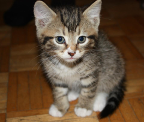
\includegraphics[width=\textwidth]{cute1}
        \caption{\underline{\hspace{2cm}}} 
        \label{fig:anzu}
    \end{subfigure}
    ~ %add desired spacing between images, e. g. ~, \quad, \qquad, \hfill etc. 
      %(or a blank line to force the subfigure onto a new line)
    \begin{subfigure}[b]{0.3\textwidth}
        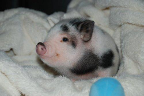
\includegraphics[width=\textwidth]{cute2}
        \caption{\underline{\hspace{2cm}}} 
        \label{fig:pig}
    \end{subfigure}
    ~ %add desired spacing between images, e. g. ~, \quad, \qquad, \hfill etc. 
    %(or a blank line to force the subfigure onto a new line)
    \begin{subfigure}[b]{0.3\textwidth}
        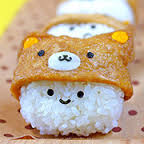
\includegraphics[width=\textwidth]{cute3}
        \caption{\underline{\hspace{2cm}}} 
        \label{fig:rice}
    \end{subfigure}   
\end{figure}

\begin{figure}[h]
    \centering
    \begin{subfigure}[b]{0.3\textwidth}
\addtocounter{subfigure}{3}
        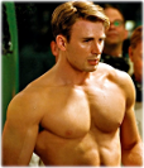
\includegraphics[width=\textwidth]{cute4}
        \caption{\underline{\hspace{2cm}}} 
        \label{fig:dude}
    \end{subfigure}
    \begin{subfigure}[b]{0.3\textwidth}
        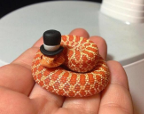
\includegraphics[width=\textwidth]{cute5}
        \caption{\underline{\hspace{2cm}}} 
        \label{fig:snake}
    \end{subfigure}
    \begin{subfigure}[b]{0.3\textwidth}
        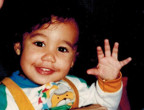
\includegraphics[width=\textwidth]{cute6}
        \caption{\underline{\hspace{2cm}}} 
        \label{fig:baby}
    \end{subfigure}  
\end{figure}
 


\newpage
\section{Visual Arts}
\subsection{Practical Applications(10 points)}
\setcounter{question}{0}
\question Draw something awesome. Preferably using more than one colour. Adherence to basic artistic principles encouraged (i.e.: complementary colours, depth, perspective, etc.)
\vfill

\newpage
\section{English}
\subsection{Multiple Choice (1 point each)}

\begin{enumerate}



\item Which sentence is punctuated correctly?

\begin{enumerate}
\item It's Lucy Liu's car, so let her decide where we're going.
\item Its Lucy's Liu car, so let her decide where were going.
\item It's Lucy Lius car, so let her decide where we're going.
\item Its' Lucy Liu's car, so let her decide where wear going.
\end{enumerate}

\item Which is an example of hyperbole?
\begin{enumerate}
\item Leeeeeeroy Jeeennnkins!
\item Oh, the weather outside is weather.
\item I have a million things to do today.
\item The vibrating washer caused the house to shake.
\end{enumerate}

\item Which poetic device is NOT being used in the following sentence:
  “Beyonce broke a bottle-BAM-CRASH-BOOM; the balcony bellowed and un-bolted itself.”
\begin{enumerate}
\item onomatopoeia
\item personification
\item connotation
\item alliteration
\end{enumerate}

\item Identify the main idea in this paragraph:

(1)You read the advertisement in the Saturday morning paper, and the deal seems too good to be true. (2)It seems that the computer you had been shopping for is available at the local computer store for half the price you found in your search. (3)You arrive at the store in the early morning, but you are greeted with a salesman's disappointing reply that the store is already sold out. (4)Still, he continues, the store can offer what you want with some upgrades for slightly more money. (5)This tactic is called bait and switch, and it is a marketing strategy used to lure customer into the store with the purpose of pressuring them into buying more than they had originally planned.

\begin{enumerate}
\item Sentence 1
\item Sentence 2
\item Sentence 3
\item Sentence 4
\item Sentence 5
\end{enumerate}

\end{enumerate}

\newpage
\subsection{Editing (10 points)}
\setcounter{question}{0}
\question The following paragraph is written poorly. Rewrite it so it is no longer appalling. Grammar and spelling are important, but so is ensuring the paragraph follows plain language rules (i.e.: the average Canadian should be able to understand the purpose of this piece.)

\vspace{1cm}

"Specially prepared for human therapeutic purposes, medicinal maggots are fly larvae. The utilization of Medicinal Maggots are sometimes referred to as "Maggot Debridement Therapy," "Larval Therapy", or "Biosurgery". Certain specie of maggots have been used -- as an alt to surgery -- to treat non-healing and infected wounds. They secrete an enzyme in order to digest necrotic tissue. Medicinal leeches are fresh water annelids that; specially prepared for Human therapeutic purposes. Theuse of medicinal Leeches is sometimes : referred to as "Hirudotherapy".  Certain species of leechs have been used by chirugeons after re-attachment surgery (such as finger reattachment) and applied to healing graft tissues to help flow. They secrete hirudin, which is a powerful anticoagulant, to do so."

\vfill

\newpage
\section{Maths}
\setcounter{question}{0}

\question[6] Determine the roots and critical points of $x^2 + x - 2$, and plot
it.
\vfill




\newpage
\question Recall that a number is said to be \emph{even} if it can be written
as $2k$, for \emph{some} integer $k$. Similarly, a number is \emph{odd} if it
can be written as $2k + 1$. For instance, $18 = 2(9)$, and $15 = 2(7) + 1$.

We can use these definitions to prove how integers change under certain
transformations. For instance, we can show that if $x$ is even, $x^2$ is even:

\begin{proof}
Because $x$ is even, we know that $x = 2k$ for some integer $k$. Therefore,
\[\begin{array}{rclr}
x^2 &=& (2k)^2 & (x = 2k) \\
&=& 4k^2 & \\
&=& 2(2k^2) & \\
\end{array}\]

$2k^2$ is an integer, so we have shown that $x^2$ is even.
\end{proof}


\begin{parts}
\part[3] Prove that if $x$ is even, $(x + 1)^2$ is odd
\vfill



\part[3] Prove that if $x$ is odd, $(x + 1)^2$ is even
\vfill


\end{parts}







\newpage
\section{Physics}
\setcounter{question}{0}

\question You fire a high-powered laser at a cat, which enters the cat's
eye. For our purposes, the eye and inside of the head can be assumed to be mostly
water.



\begin{parts}
\part[1] What law governs how the beam of light will behave when it enters the
cat's eye?
\\
\\

\part[2] Assuming the surface of the cat's eye is perpendicular to its brain,
do you expect the beam of light to bend towards the cat's brain and destroy it,
or bend away and save it? Why?
\vfill
\end{parts}





\newpage
\question[9] You plan to fire a cat from a trebuchet. Based on your calculations, the cat
will leave the trebuchet at a height of $4m$, travelling $10m/s$, at an angle of
$45$ degrees from the ground ($cos(45) = sin(45) = 0.7$). The cat weighs $1kg$,
is spherical, uniform, frictionless, and a perfect conductor. Gravity is $10m/s^2$

How far from the trebuchet should you place your lava pit to catch the cat? Note
that your lava pit is fairly large, and cats are dumb and will probably run into
it anyway, so precision isn't particularly important (i.e. feel free to approximate square
roots). We're more interested in
your methods.







\newpage
\question[3] Albert Einstein and Isaac Newton are in a fist fight. Each uses their
mastery of physics to amplify their blows. Einstein uses general relativity to
make his fists twice as massive on impact. Newton uses gravity wells to make them twice as
fast (but still punches as frequently). Who has the advantage, and why?
\vfill





\question[3] Bonus: If Newton's and Einstein's fists have a resting mass of 1kg and
originally punched at $1/10$th the speed of light, how does this change the situation?
\vfill

\newpage
\section{Bonus Round! (1 point each)}
\setcounter{question}{0}
\question What famous hockey player signed the inside of Matt's miter board when he graduated high school? 
\vspace{2cm}
\question Write a haiku.
\vspace{5cm}
\question What's your favourite alchoholic drink? 
\vspace{2cm}
\question If purple had a smell what would it's square root be? 
\vspace{2cm}
\question This hit / That ice cold / Michelle Pfeiffer
\vspace{2cm}


\end{questions}
\end{document}
